\documentclass{elsarticle}
\usepackage{amssymb}
\usepackage{amsmath}
\usepackage{bigdelim}
\usepackage{multirow}
\usepackage{hyperref}
\usepackage{graphics}
\usepackage{algorithm}
\usepackage{algorithmic}
\usepackage{subfigure}
\usepackage{booktabs}
\usepackage{url}
\usepackage{natbib}


%\usepackage{algorithmicx}
\journal{International Journal of Human-Computer Studies}

\newtheorem{definition}{Definition}


\begin{document}

\begin{frontmatter}
\title{A system dynamics analysis of motivation factors of knowledge collaboration in VCoP}
\author[buaa]{Jun Wang}
\ead{king.wang@buaa.edu.cn}

\author[buaa]{Yunpeng Wu}
\ead{yunpeng.wu@sem.buaa.edu.cn}

\author[buaa]{Di Wu}
\ead{sss}

\address[buaa]{School of Economics and Management, Beihang University, 
Beijing 100083, P.R. China}

\begin{abstract}
 With the development of Virtual Community of Practice (VCoP), a lot of research was done on the mechanism and structure of virtual community, while little research was about the motivation of users’ behaviors. Based on achievement motivation theories and community theories, the motivation factors of users to participate knowledge collaboration are elaborated from individual and group environment perspectives. For further explanation, we developed a dynamic model to simulate the motivation factors of users in VCoP, which was compared with the historical data from Wikipedia,. Finally, based on the simulation and analysis results we propose the strategy to improve the virtual community development and the future study. 

\end{abstract}

\begin{keyword}
  Virtual Community of Practice, System Dynamics, Motivation Factors, Achievement Motivation, Sense of Community, simulation model

\end{keyword}
\end{frontmatter}

\section{Introduction}
\label{sec:introduction}
Morden information technology enables people to communicate in a way
even not having to meet each other. Online communication gradually changes the
traditional communities to virtual communities.  A sufficient number of
people  aggregate in cyberspace and participate in  an open discussion
long enough, with sufficient emotions, setting up  their personal
relationship\cite{rheingold2000vch}. This kind of community is also
named as online community and computer mediated community. While
virtual communities may seem common to people's daily life,
researchers of knowledge management find virtual communities are great
form to better share and transfer knowledge in organizations. Member
of these communities in an organization focus their eyes on certain
topics, keep learning and practicing,  which forms virtual
communities of practice(VCoP). 

The connections between members of  VCop are relatively weak since VCoP is
self-organized and self-maintenance. People join and quit the
communities freely at their own will. However, people keep on
attending the practice activites with great passion under such week
connections, without explicit reward from communities. Scholars and
organization managers are interested in finding what impact factors drive
people to contribute their effort and enthusiasm into the communities,
that is, what are their motivations.

Motivation is the dynamic factor formed by individuals collaborating the internal requirements(such as instinct, need and drive) and external cause of behavior(such as goals, reward and punishment), which can inspire and maintain the behaviors.
Sociologists and psychologists firstly studied some kinds of virtual
communities, such as online-shopping community and consumption community
modeling the internal and external impact factors and how they affect
people's behavior\cite{teo1999iae}\cite{shang2005evi}. This is because
the motivation  driving users to participate virtual community of
practice is mostly social and  psychological  motivation. Several
behavior  models
are adopted in theses studies and discuss the factors from management,
pedagogy and psychology perspectives.

Though different schoalrs gave different impact factor of motivation
using different models in differnt communities, few of them studied
what are the interactions between these factors and how these factor
take effect together. The motivation of members in virtual community is
a systematic problem involving personal influence factors, group
influence factors and the relationship between different factors, and
its practical results are decided by interaction of those factors. The
impact factor should not be seen as independently affect members'
behavior in VCoP, nor their effect will last at a certain level in a
long duration. A model can describe the impact factors interaction and
predict the change of their effect is indispensable for study of
VCoP. 

In this paper, we adopt system dynamics as our modeling
tool. The fundamental of system dynamic modeling is its systems view
and the unique process of recognizing and the solving problems from
unity to part and from outside to inside with manifold
loops. System dynamics attaches great importance on the complicated
requirements in decision making process and the cognition process
generated naturally or by the education. Recently, an increasing
number of scholars have accepted system dynamics as the tool in
virtual community research. For example, Diker  developed a
membership growth model in an open online system\cite{diker2004dynamic}. Mao etc build a system dynamics model of an online collaborative system and studied
its motivation mechanism\cite{4076734}. Wittmann and  Hattrup
adopted system dynamic to create a feedback model for information
overload\cite{wittmann_relationship_2004}. Tina presented a system dynamics model of
the evaluation system of educational techniques\cite{stavredes2001system}. Consequently, it is natural to choose system dynamics to
research the motivation factors from personal requirement and
organization environment perspectives. we developed a system dynamics model to simulate the motivation factors, where the individual psychological factors and the group influence psychological factors are mainly studied. In this model, the cause and effect relationship and the influence factors need to be verified and modified constantly, and this can be realized by computer technology and simulation software, which also helps to identify the complicated relationship between the system factors and the system structure. 
 
The paper is organized as follows: The next section discusses the
classification of members in VCoP. Section 3 analyzed the motivation factors
in VCoP. In section 4 we modeling the factors based on system dynamic
to show the causality of the factors and members behavior. In section
5 we do a simulation based on data Wikipedia community to verify our model.  Finally, the contributions and limitations of this study, and implications for future research are discussed.






\section{The classification of members in VCoP}
\label{sec:classification-uses}

Members in virtual community of practice will organize themselves to work and learn together in a certain field, and achieve some goal by communication and knowledge sharing. Essentially, it is a process of knowledge collaboration and knowledge-based task performance. 

Not all members in VCoP stand at same levels. Not only because of  different personalities, motivations,
behaviors and qualifications, various levels of activeness,
characteristics, ability of expression, knowledge, but more important, roles in
community interaction. users in the same virtual community will be
differentiated in the sense of community and grouped spontaneously. 

Amsrtnog and Hgael(1997) classify the members into 4 categories from
content contribution perspective. In VCoP, individuals are attracted
by topics they are interested in before they devote themselves to the
related community. Inclined to join the community as they are, whether
they can be converted from simple browsers to community users who will
enter the community repeatedly, interact with others and contribute
knowledge, depends on the amount of their interest and
satisfaction. According to dimensions of participation and value to
the community, Amsrtnog and Hgael divided virtual community members  into: browser, lurker, contributor and shopper. Adler and Christopher(1998) presented the four types of users as passive member, positive member, inductor and manager[20]. After a long time of observation of game-programming MUD virtual community, Bartle(1990)classified the users as killers, achievers, socializes and explorers according to their motivation and related behaviors. Kozinest(1999) , when studying the consumer virtual communities, divided the members as tourist, mingler, devotee and insiders based on the relationship between users and consuming activities and relationship between users and virtual communities. According to Kozinest, the final identification depends on two related factors: the degree of the relationship between individuals and certain consuming behaviors, and the social relation between individuals and other members in the community. According to the two factors, community members can be divided as four types shown in figure 1.   
\begin{figure}[htpb]
  \centering
  \scalebox{0.75}{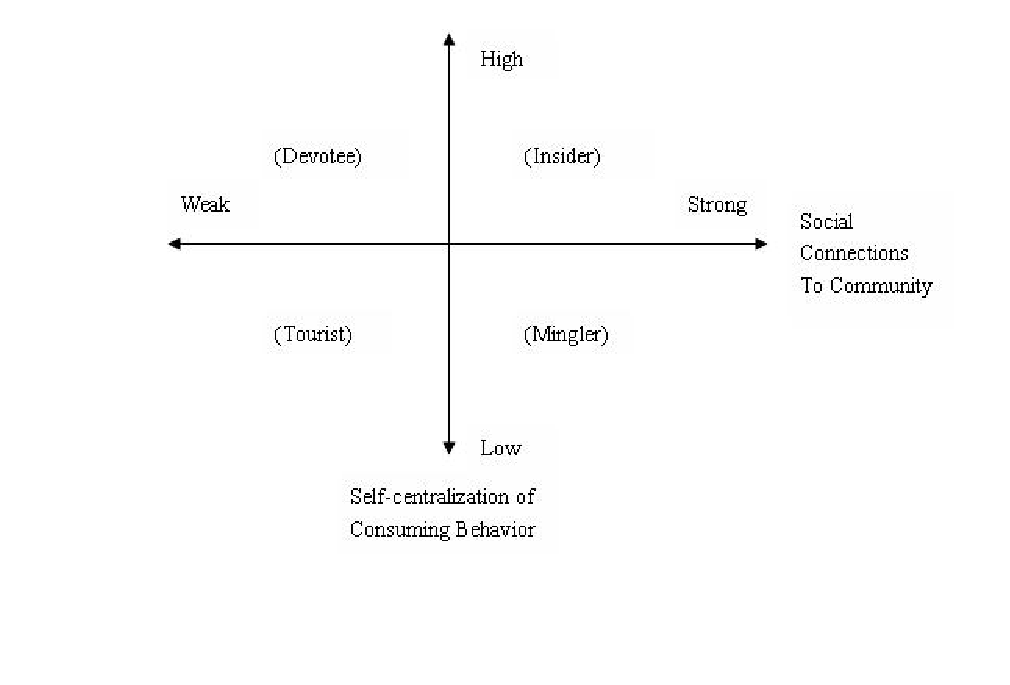
\includegraphics{01}}
  \caption{Classification of members in VCoP}
  \label{fig:classification}
\end{figure}


\begin{enumerate}
\item Browser: lack of intense social relationship with groups; having
  temporary or little interest in consuming behavior. 
\item Mingler: intense relationship with groups; but little interest in core consuming behavior.
\item Devotee: enthusiastic with consuming behavior,; weak
  relationship with groups. 
\item  Insider: intense relationship with consuming behaviors and groups. 
\end{enumerate}


As a special kind of virtual community, VCoP has some unique
characters which differentiate it form other communities. Firstly,
practices are the main activities in VCoP and the outputs of practices
are much more definite and explicit. Participants actively dive into
practices and knowledge transfer and sharing occurred in the
practices. This characteristic make the relationships between members
in VCoP are primarily "mentorship". This kind of connections involve
two subjects:
\begin{itemize}
\item  knowledge providers: Those who are knowledgeable and willing to
  provide their knowledge by presentation, works and behaviors. They
  either provide the related knowledge to solve the problems presented
  by other members, or post messages in the community to introduce
  their experience and techniques. In the collaboration process,
  knowledge providers contribute their own knowledge to the community
\item  knowledge requestors: knowledge receivers. Those who learn and understand knowledge by imitation, listening and reading. Knowledge requestors acquire the knowledge they need in the collaboration process.
\end{itemize}
Members master some skills from
learned people in practice activities. The roles change rapidly in
VCoP, once the browser members gained enough knowledge in communities,
usually they become insiders to lead other browser members to take
part in practice activities22. On the contrary, building human
relationships are not primary goals for VCoP members.  In this paper,
we classify the members in VCoP into two categories because of the
relatively pure and simple relationship:   Experienced members and  ordinary members.

(1)  Experienced members: Experienced members are opinion leaders with highest influence. They are most familiar with the related information and knowledge, also they are willing to interact with others and provide their assistance. Generally, they are the most passionate and active members in the community, not only contributing their original product but also organizing or participating in discussions or activities as much as possible. 

(2)  ordinary members: ordinary members are members who just
participate in the community and those browsers. The former, lack of
strong social relationship with others, usually browse casually and
contribute little to the community. Moreover, they are inclined to
dive in the community, and obtain the knowledge they need without much
contribution. The browsers mean tourists who browse and learn in the
community with little contribution to it. 

We see the  experienced members roughly equal to insider and
devotee. Most of the contribution to VCoP are from their effort. They
lead the practices in VCoP, participating in the activities or
discussions initiated by others, and then offering his advice and
methods.Also they play mediating roles between community members and community operators, in charge of everyday concerns.
 The ordinary members equal to browser and lurker. They are followers
 to experienced members and make little contribution due to lack of
 knowledge and unfamiliar to community culture. Acquiring knowledge
 from others passively by take part in practices are their normal activities.



\section{Motivation factors analysis of knowledge collaboration in virtual community of practice}
\label{sec:motiv-fact-analys}


 Dholakia et al. \cite{Dholakia2004241}divides the users’ motivation to participation as two sorts: One is the motivation on the individual level, including achieving goals, maintaining social relationship, social reinforcement and entertainment; The other is the motivation on the group level, including internalization and recognition. It refers to the social influence factors affecting the members’ participation in the virtual community. Therefore, we study the motivation factors affecting the members’ participation in the virtual community from two aspects: on the individual level and group level.  

\subsection{Individual level motivation factors}
\label{sec:individual-level}

Motivation can be basically categorized into intrinsic motivation and
extrinsic motivation considering their "origin". Intrinsic motivation
inherently  stems from individuals themselves, referring to doing something because it is interest-
ing or enjoyable. Extrinsic motivation refers to doing something
because it leads to a separable outcome.  It focuses on the efficacy
of the activities, which are regarded as a tool to achieve the goal. Piles of research have
shown that the different quality of experience and performance can be achieved
when one is behaving for intrinsic versus extrinsic
reasons\cite{Ryan200054}.  Extrinsic motivation is generated by
objective factors other than individuals themselves. It focuses on the
efficacy of the activities, which are regarded as a tool to achieve
the goal. Besides, extrinsic motivation can be observed and felt and
it is acquired by the exchange of material, energy and
information. Intrinsic motivation stems from individuals themselves
and involving in the activities without any effect of external
force. It focuses on the process of activities instead of the
efficacy, including sense of responsibility, sense of achievement and
need for achievement, and so on. 

Intrinsic and extrinsic motivation have different effect to motivate people\cite{deci1985ima}. A large quantity of empirical studies have proved the important role
of extrinsic motivation. However, it is hard to determine which factor
takes the priority, Furthermore, some of virtual communities solely 
developed by the enthusiasm of users instead of extrinsic
rewards. Therefore, intrinsic motivation is as important as extrinsic
motivation. Intrinsic motivation is generated from the altruism of
individuals and the satisfaction of the psychological needs, or from
the pursuit of some certain moral principles. Intrinsic motivation is
mostly the satisfaction of some certain psychological
needs\cite{josh_lerner_simple_2002}. In this paper we propose 
the extrinsic and intrinsic 
motivation factors on the individual level  as the
follows: 


\subsubsection{ Information value}

Information value contains acquiring
  information, learning to handle affairs, providing information and
  contributing all the knowledge to a pool of
  information\cite{flanagin2001internet}. Dholakia studied some of the individual factors, finding that the
informational and instrumental value is the vital
factor to motivate people attend the communities\cite{Dholakia2004241}. Information value is not only the result of
  virtual community of practice but also the primary factor of members
  to participate in the community. Davenport etc points out that it is like Utopia to think that
knowledge will naturally distribute without economic incentives,
because people are not likely to contribute valuable knowledge without
any returns\cite{davenport1998wko}. Individuals will not be interested
  in other factors of the virtual community unless they could obtain
  the related information to meet their needs for knowledge.

  \subsubsection{Instrumental value}
\label{sec:instrumental-value}
  
Participating practices in VCoP will bring certain particular value or
be conducive to a final value\cite{Roennow-Rasmussen2002}. 
Participants will complete a certain task through
online interaction, such as solving a problem, providing an original
view, affecting others, and evaluating a decision. These tasks are all
instrumental, which is often defined as the easiness to achieve the
specific goals. Flnagani and Metgze argue that instrumental
value(instrumental need) means view generation, negotiation, problem
solution, finding others for assistance and decision making\cite{flanagin2001internet}.

\subsubsection{Extrinsic rewards}
\label{sec:extrinsic-rewards}


   Generally, in virtual communities the rewards are
  not presented in material. But larger personal spaces and more
  privilege for functions have become the extrinsic motivation factors
  for users to participate in the community practice.  More
  importantly,  praise from other members and
honorary recognition will bring great satisfaction which compensate
their effort dived into the communities, in turn motivate them keep
attending the practices\cite{Zhugea}.

\subsubsection{Reciprocity}
\label{sec:reciprocity}

Everyone is limited to his abilities. Acquiring knowledge form others
is becoming more and more frequent because of the complexity of tasks
or problems. People sharing their knowledge have the expectation that
they will gain knowledge payback.  Usually, reciprocity is not realized simultaneously, but the
efficiency could be improved by interaction and mutual assistance.

\subsubsection{Need for achievement}
\label{sec:need-achievement}


 It means the individuals’ requirements for
success and best performance. Nicholls(1982)discovers the intrinsic
dynamic for people to strive for success when they are performing a
task, that is, the inner drive for people to do those tasks perceived
to be important and valuable. It is defined as achievement
motivation. Clark、Varadarajan and Pride also take achievement
motivation as the competition for excellence or the hope for realizing
one’s goals[32]. Clark etc. take achievement motivation as the competition for
excellence or the hope for realizing one’s goals\cite{clark1994emc}. 
Elliot also argued  the achievement motivation is the
competition-based emotion, cognition, activation and orientation of
behaviors\cite{elliot1999aaa}.  McClelland argues that people
with strong need for achievement aspire to do things in a perfect way,
improve working efficiency and become more successful\cite{mcclelland1976am}. They are
concerned with the joy in overcoming difficulties, solving problems
and the sense of achievement after success, but material award is not
their concern. The sense of achievement is closely related with the
standard of economics, culture, society and government, as well as the
social moralities. The sense of achievement of individuals is
satisfied in the practice, which inversely encourages the individuals
to participate in the virtual community. 

\subsubsection{ Need for power}
\label{sec:need-power}

It is the requirement of affecting or controlling
others without being controlled. Also, it refers to the drive to
control and influence others. The extent of aspire for power
varies. Those who are endowed with a strong aspire for power are
interested in controlling, ordering, and claiming for
power. Correspondingly, they are typically argumentative, talkative,
straight, and clear-minded; they are born instructors and
lecturers. They pursue excellence and competitive environment not for
the sense of achievement as those with strong need for achievement,
but for acquiring power and status or maintaining the present
power. One kind of participants, called community leaders in virtual
community, whose advice can influence other members to a great degree,
will make lectures and instruct others when there is a debate, and
later they will obtain higher status and power in the community. 

\subsubsection{ Need for affiliation}
\label{sec:need-affiliation}

It is the need to establish intimate social
relationship, and a desire to seek for being loved and
accepted. People with strong need for affiliation are fond of
associating with others, which brings joy to them. Sensitive to
interpersonal relationship, they prefer cooperative to competitive
working atmosphere, and need more communication and mutual
understanding. Sometimes, this kind of need is presented as the fear
to lose intimate relationships and the withdraw in front of
interpersonal conflict. In virtual communities, the need for
affiliation is important to keep social association and harmonious
interpersonal relationships.

\subsubsection{Self-efficacy}
\label{sec:self-efficacy}

It is an significant intrinsic motivation which
helps to initiate knowledge collaboration between community
members.  Within personal
achievement, self-efficacy is a vital category which is defined as
“Individuals’ perception or belief of their ability to control the
life” \cite{bundura1977slt}. He discovers that the act of individuals not only depends
on their willpower but also on their self-assurance of the effective
use of power, which can be realized by self-efficacy. As a latent
important factor affecting knowledge collaboration, self-efficacy is
the belief of the organization and execution ability needed for the
expected condition. In the context of achievement, self-efficacy is an intuitive
or personal judgment made by an individual on whether he is competent
for the task before undertaking it. It is both self-perception of
competence and an emotional private experience. After studying the
motivation factors for workers to contribute knowledge to enterprise
knowledge base,  Kankanhalli believes that the motivation will be
weakened if the workers think their knowledge has no effect to the
enterprise. Hsu gets the similar conclusion after studying the
motivation factors of knowledge sharing in virtual community:
Self-efficacy is an important motivation of knowledge sharing.

\subsection{group level}
\label{sec:group-level}

Virtual community is a social group formed by the aggregation of online users Since the sociality is a typical feature of virtual community, social factors are crucial in motivating members to participate in virtual community. The sense of community, which is a combination of the sense of belonging, sense of identity, emotional connection and the feeling of stability, reflects the need for others and the interaction with others of each individual. Furthermore, there will be active impact of the sense of community. Mcmillan and Charvis presents the most influential and typical definition of the sense of community, that is, the sense of belonging, the perception of important relationships and community significance, and the common belief that the group is obliged to meet the members’ needs\cite{mcmillan1986scd}. Although there is no face-to-face interaction and regional association in the computer-based virtual community, the sense of community will be generated from it. The anonymity (the real identity will not be exposed) and selectivity (people can enter or leave the community at any time) enables people to explore themselves and build identity more freely, thus brings a more interactive and open society. Therefore, virtual communities could meet the needs of sense of community that can not be satisfied in real communities. In this study, we define community identity, community attachment, community cohesion, and community satisfaction as four fundamentals of the sense of community in virtual communities.      

\subsubsection{Community identity}
\label{sec:community-identiy}

community identity involves the semiotic significance and social value for people, that is, the process and extent of the community becoming the self-identity of individuals, which seems like the sense of membership. Sense of identity is the extent individuals feel themselves as part of the group. The extent of the sense of identity varies with different individuals or groups, and the sense can be analyzed in cognitive, afflictive and evaluative aspects\cite{warren1972ca}. Dholkaia argues that the sense of identity includes cognition, affiliation and evaluation\cite{dholakia2004sim}. From the view of cognition, identity is a process of classification, which means the extent of individuals’ recognition of themselves as a member in the virtual community.(similar with the members and different from non-members) ; From the view of affiliation, identity means the emotional state of belonging to a virtual community; Evaluation is what users evaluating themselves in the virtual community.    

\subsubsection{Community attachment}
\label{sec:community-attachment}

Community attachment is the emotional engagement in the community which is similar with “mutual emotional relationship”. The individuals participate in virtual communities to escape from loneliness and communicate with people of the same thoughts, obtaining friendship and social support. The members will tend to participate owning to their sense of the membership. Postmes argues that the attractiveness of virtual communities comes from the sense of cluster, which is a positive experience of members gathering together to communicate with each other in the virtual community\cite{t_postmes_formation_2000}.     

\subsubsection{Community cohesion}
\label{sec:community-cohesion}

community cohesion emphasizes on the group interaction and the
unity between individual goals and group goals, which seems like
“influence” and “the integration and realization of needs”. There is
an phenomena named internalization in community cohesion. The
internalization means making decisions based on the overlap between
one’s sense of worth and others’. Eagly and Chaiken indicates that the
sense of worth cover a large quantity of concepts, such as belief,
attitude and other moral belief\cite{eagly1993pa}. For members in the virtual
community, internalization happens when they share the same sense of
worth with others. In the virtual community of practice, an expertise
in java may meet others who like java as he does, or a fan of
archaeology will meet with other fans who are posting their comments
on the relate topics. In every condition, there is some apparent
overlap of the sense of worth. Owning to the casualness of selection,
that is, community members could select the virtual group that share
the same sense of worth with themselves, Bagozzi and Dholakia(2002)
view internalization as an important influential factor of community
members\cite{richard_p._bagozzi_intentional_2002}. Internalization develops in the information exchange among
community members and keep growing when the information means a lot to
the participants. 

\subsubsection{Community satisfaction}
\label{sec:comm-satisf}

Community satisfaction is an emotional state of community
evaluation. It is also close to community cohesion, referring to the
subjective evaluation of the objective condition in the community. The
research on community satisfaction made by Malans and Jess(1975) is
the most prominent one. They find that the features of the objective
condition where an individual lives are not equal to his feelings in
that condition. Most people, even those living in a lower standard are
satisfied with their community. In most circumstances, satisfaction is
highly related with the affiliation to the family and the friends
living in the community\cite{marans1975tuc}. John Buckner, the psychologist, presents
a research of studying community (cohesion) sense on the group level,
and presents three dimensional indexes measuring the neighborhood
cohesion: the sense of community of residents in the neighborhood, the
livings of residents and the level of residents’ attractiveness to
other neighbors, and the level of interaction with
neighbors\cite{buckner1988dim}.

The individual level motivation factors are presented in table \ref{tab:individual-level}.

\begin{table}[htpb]
  \label{tab:individual-level}
  \centering
   \caption{the classification of motivation factors for the virtual
    community members to participate in knowledge collaboration}
\begin{tabular}{ccc}
    \toprule
    \multicolumn{ 1}{c|}{Individual level} & \multicolumn{ 1}{|c|}{extrinsic motivation} & Information value \\
    \multicolumn{ 1}{c|}{} & \multicolumn{ 1}{|c|}{} & Instrumental value \\
    \multicolumn{ 1}{c|}{} & \multicolumn{ 1}{|c|}{} & Extrinsic rewards \\
    \multicolumn{ 1}{c|}{} & \multicolumn{ 1}{|c|}{} & Reciprocity \\\cline{2-3}
    \multicolumn{ 1}{c|}{} & \multicolumn{ 1}{|c|}{Intrinsic motivation} & Need for achievement \\
    \multicolumn{ 1}{c|}{} & \multicolumn{ 1}{|c|}{} & Need for power \\
    \multicolumn{ 1}{c|}{} & \multicolumn{ 1}{|c|}{} & Need for affiliation \\
    \multicolumn{ 1}{c|}{} & \multicolumn{ 1}{|c|}{} & Self-efficacy \\\hline
    \multicolumn{ 1}{c|}{Group level} & \multicolumn{ 2}{|c}{Community identity} \\
    \multicolumn{ 1}{c|}{} & \multicolumn{ 2}{|c}{Community attachment} \\
    \multicolumn{ 1}{c|}{} & \multicolumn{ 2}{|c}{Community cohesion} \\
    \multicolumn{ 1}{c|}{} & \multicolumn{ 2}{|c}{Community satisfaction} \\
    \bottomrule
    \end{tabular}
\end{table}

 

\section{The causality of motivation factors and human behavior}
\label{sec:modeling-process}

There is a mutual supportive or restrictive relationship between the
intrinsic and extrinsic motivation on individual level, and the same
relationship exists between the individual level and group
level. Dholakia discovers that the target value of t=individuals will
strengthen their sense of identity, which brings the common sense of
members resulting in the community cohesion\cite{dholakia2004sim}. David Mcmillan and David
Chaves argue that the common experience and interaction embodies
important psychological rules. ① Association hypothesis : The more
people interact with each other, the more intimate they will be. ②The
quality of interaction: The more active the experience and
relationship is, the more close the relations will be; Achievements
promote cohesion. ③ Behavior prevention: Uncertain interactions and
the non-completion of community tasks will prevent the community
cohesion. ④The hypothesis of equivalent events: the greater events
people have experienced together, the closer connections will be. (For
example, people will get closer connection if they have experienced a
catastrophe together); ⑤Devotion: The devotion determines the
importance of the history and current situation to community
members(For example, the one who devotes more to the community will
feel the impact of community events more easily; Also he will have
more affection on the community); ⑥The influence of the honor and
humiliation on community members: The honor and humiliation is very
influential on the members’ attitude on the community. ⑦Spiritual
connections: connections generated or strengthened by common
spirit(such as the religion and racism)\cite{mcmillan1986scd}. Bagozzi and
Dholakia(2002) finds out the sense of identity will increase the
individuals’ desire, which is reflected as various psychological
requirements, when they are moderating the MGB model. Moreover, active
emotion expectations will increase the individuals’ psychological
desire\cite{richard_p._bagozzi_intentional_2002}. Based on the analysis, we conclude the basic
cause-and-effect relationship between motivation factors in virtual
communities of practice shown as figure 2.
\begin{figure}[htpb]
  \centering
  \label{fig:cause-and-effect}
  \scalebox{0.8}{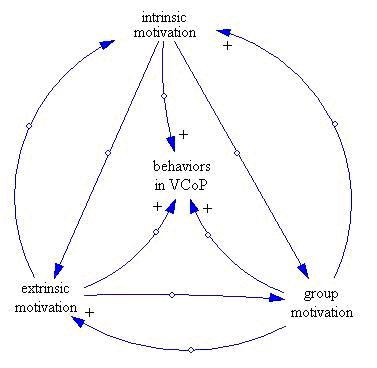
\includegraphics{02}}
  \caption{虚拟实践社区动机因素基本因果关系}
\end{figure}

\subsection{The motivation factor model of experienced members}
\label{sec:motiv-fact-model}

 Experienced members in virtual community of practice mainly
 participate in the collaboration and discussion, but rarely browse or
 manage in the community. Therefore, in this model the behavior
 dimension includes two horizontal variables: collaboration and
 communication. 

   On the individual level, experienced members will focus on the
   instrumental value of the community and the extrinsic rewards will
   have effect on some of them. Reciprocity is also meaningful for the
   experienced members. Because they join the collaboration mainly for
   solving problems instead of acquiring information, the information
   value of the community is not very distinct. In general,
   experienced members have stronger need for achievement, and some of
   them have stronger need for power or need for affiliation. They
   would like to undertake the responsibility and complete the task
   with some achievement, so their self-efficacy is higher and has
   positive impact on themselves. On the group level, experienced
   members have become regular members in the community, with their
   sense of identity, belonging, cohesion, and satisfaction at a
   higher level. Those psychological factors will correspondingly
   prompt them to participate in the collaboration more
   frequently. Consequently, the motivation factor dimension includes
   11 horizontal variables: instrumental value, extrinsic rewards,
   reciprocity, need for achievement, need for power, need for
   affiliation, self-efficacy, community identity, community
   attachment, community cohesion, and community satisfaction. The
   motivation factor model of experienced members is shown as figure
   3.
\begin{figure}[htpb]
  \centering
  \label{fig:senior member}
  \scalebox{0.8}{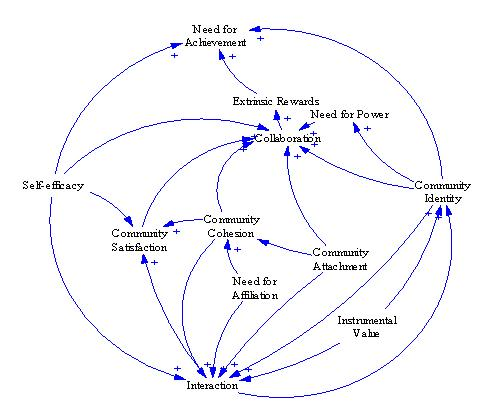
\includegraphics{03}}
  \caption{Model of motivation factors for senior
    member in VCoP}
\end{figure}

\subsection{motivation factor model of common members}
\label{sec:motiv-fact-model-1}

Common members in virtual communities take no activity except browsing, which is the only horizontal variable in the behavior dimension in this motivation factor model of common members. 

On the individual level, common members often lay great emphasis on
the information value and instrumental value of the community in
practice. Without undertaking any tasks, there is rarely any extrinsic
rewards and reciprocity between members. Although there are only a few
common members who contribute little to the community, there is some
latent need for achievement and need for affiliation. And there is
little need for power among them. Because their behavior is mainly
browsing that is seldom affected by self-efficacy, the horizontal
variables do not involve self-efficacy in this model. On the group
level, the common members’ sense of identity, belonging, cohesion and
satisfaction is weaker compared to the experienced members, but these
psychological factors will spur them to participate in the
collaboration. Therefore, the motivation dimension includes 8
horizontal variables: information value, instrumental value, need for
achievement, need for affiliation, community identity, community
attachment, community cohesion, and community satisfaction. The
motivation factor model of common members is shown as figure 4.  
\begin{figure}[htpb]
  \centering
  \label{fig:common-member}
  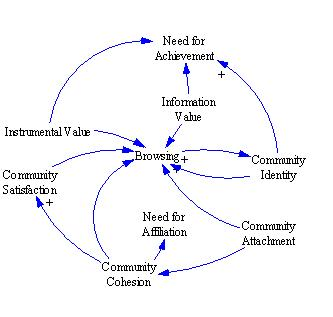
\includegraphics{04}
  \caption{Model of motivation factors for common
    members in VCoP}
\end{figure}

\section{Simulation research }
\label{sec:simulation-research-}

 Based on the basic model, we moderate the model according to
    Wikipedia, and make a system simulation research. A contrastive
    analysis is made between the simulation results and the real
    data. 

\subsection{The background of simulation research: Wikipedia}
\label{sec:backgr-simul-rese}
Nowadays Wikipedia has been the world largest online
encyclopedia. Millions of people work together to add content to it
even without knowing each other. Wikipedia provides a few easily
handled tools allowing people edit the content collaboratively. People
of different background join the community to complete comprehensive
and accurate articles. Thus we see Wikipedia is a good example of VCoP
for our study 
  We choose Wikipedia as our case study, and make simulation analysis of the motivation factors for users to participate in knowledge collaboration. 

Wikipedia foundation provides comprehensive data archive to download
for scholar research. In this paper, we choose Chinese edition of
Wikipedia as our research
target\footnote{http://download.wikimedia.org/zhwiki/20090714/}. The
unique characteristic Chinese Wikipedia community has is "honor and
award of Wikipedia" to praise the volunteers for their great
effort. This mechanism  has carried out for a long time since 2005, so
there could be enough extrinsic motivation for every participant. 
   

A system is an functional aggregation with distinct and interactive parts connected together. We should first define the boundary of system and make primary feedback analysis before the system dynamics model could be built. Users edit entries through the behavior of edit, and communicate with each other through the behavior of Talk. This study describes virtual community of practice in two perspectives: a) the result of users’ practice; b) the psychological factors prompting the generation of practice results, including factors on the individual level and group level. In wiki, users collaborate with each other by editing entries and they can talk with each other about entries and texts of questions. Individuals complete editing entries voluntarily without any extrinsic rewards, which indicates that users in wiki are endowed with the similar and strong self-efficacy. The basic concept model includes Edit, Talk, need for achievement and the sense of community. The constant participation behavior of users influenced by individual and environmental factors is featured by positive feedback and the tendency of self-reinforcement. The moderated model is explained by the cause-and-effect graph shown in figure 5. 

\begin{figure}[htpb]
  \centering
  \scalebox{0.65}{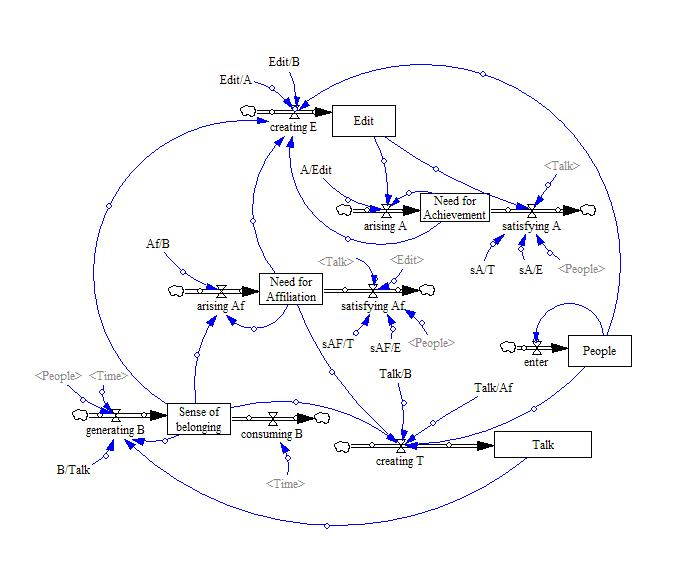
\includegraphics{05}}
  \caption{sds}
\end{figure}
\subsection{The definition of factors in the Wiki system simulation model
}
\label{sec:defin-fact-wiki}

In wiki, users collaborate with each other on a question and they can talk with each other about questions and texts of other topics. In this study, we adopt need for achievement and the theory of sense of community to explain the psychological factors driving community members to collaborate and communicate with each other. Based on the basic cause-and-effect graph, we make further feedback analysis on the motivation factors for community users to participate in knowledge collaboration, and define the horizontal variables of the system dynamic model of motivation factors in wiki as 
Level 1 Edit: The way in which users participate in practice. As an open community, the virtual community of practice allows users to collaborate with each other by creating and moderating entries. In editing, which is an equal collaboration, each member has the identical power and responsibility. The knowledge collaboration is completed by the edit of entries or categories, thus edit is treated as a horizontal variable of this study. 
Level 2 Talk: The way in which users communicate with each other. The communication through text among members in virtual communities reflects the coordination and affiliation between the members. Because users could discuss and exchange ideas on entries and categories through Talk pages, Talk is included as the horizontal variable indicating the communication between members. 
Level 3 Need for achievement: Meclelland believes that people with strong need for achievement aspire to work more efficiently and struggle for greater success. They are not concerned with material rewards. This sense will increase with personal achievement and decrease for some other reasons, such as the attribution and comparison, so the need for achievement is defined as a variable in this study.
Level 4 Need for affiliation: The need for affiliation and the shared
emotional connections in the sense of community indicates that members
can reduce the personal distance between them by communication and
establishing intimate social relationships. With the increasing level
of intimacy between individuals, the community cohesion will be
strengthened, and it will also be weakened owning to the community
policy. Consequently, we define the need for affiliation as the
horizontal variable.  
Level 5 Sense of belonging: The sense of membership includes 5 factors: Boundary, sense of security, sense of belonging and identity, personal investment, and the common semiotic system. In the virtual community, there are open boundaries, the sense of security with little impact on the open community, the personal investment which could be reflected by knowledge collaboration and the common semiotic system defined by the system itself. Therefore, only the sense of belonging can be defined as the horizontal variable reflecting the membership in the community.
Level 6 People: The individual is an important factor of the community constitution, and it is defined as the horizontal variable in this study. 
Collaboration in Wiki emphasizes on the equality and coordination of
the relationship between numbers. Consequently, there is no community
leaders whose power transcend other individuals, thus, there is no
need for power and no desire for leadership in the community. Though
McMillan and Chavis take influential power as the most important
factor in the sense of community, Anita L. Blanchard discovers strong
relationship between members and weaker individual impact, and
furthermore, the exchange and support between members is significant
for the community development [45]. Some other scholars also prove
that the influence in the sense of virtual community is not as
important as SOC. As a result, we do not include influential power as
a factor. 

\subsection{Wikipedia系统仿真模型结构优化}
\label{sec:wikipedia}

McMillan and Chavis argue that the common experience and interaction
of community members reflect important psychological activity
rules. Moreover, they find that more interaction will bring higher
intimacy, and more active relationship promotes closer
connection. Cohesion is strengthened by achievement, while investment
determines the significance of the community to members. The sense of
community becomes stronger with larger investment. Influenced by
individual and environmental factors, users participate in the
practice constantly, so the 5 horizontal variables are mutually
promotive and featured by the self-reinforcement of positive
feedback. Figure 6 describes the moderated motivation factor model of
users to participate in knowledge collaboration according to real data
from wiki.

\begin{figure}[htpb]
  \centering
  \scalebox{0.7}{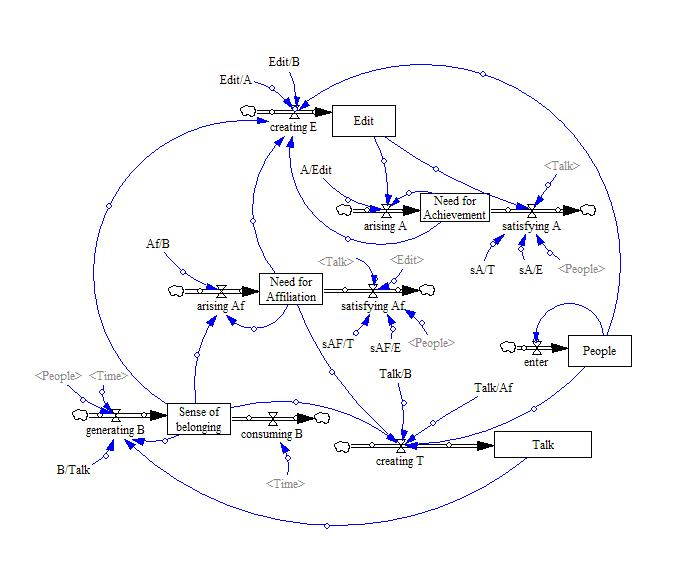
\includegraphics{06}}
  \caption{sfd}
\end{figure}

Based on the previous analysis of the effect of intrinsic motivation
on behavior, the users’ knowledge will accumulate in practice, at the
same time, their need for achievement and affiliation will grow until
it becomes stable. The input stream that influences the need for
achievement and the need for affiliation is defined: Arising A and
Arising Af; The motivation itself will also not grow infinitely, so
two output streams are designed for need achievement and need for
affiliation: Satisfacting \underline{xiahuaxian} A, Satisfacting Af. As time goes on,
members’ sense of community will grow with the increase of knowledge
collaborators, so the input stream of sense of belonging is defined:
generating B. According to psychology principles, the human feelings
will decay as time goes on, and the output stream of sense of
belonging is defined as: consuming B. The details of variables and
parameters are shown as table 2. 
\begin{table}[htpb]
  \centering
 
  \caption{ the variables and input/output parameters in system
    dynamic model}
\begin{tabular}{c|c|c|c|c}
   
    \toprule
    \parbox{1.5cm}{horizontal variable} & \multicolumn{ 2}{|c}{\parbox{2cm}{input stream params}} &
    \multicolumn{ 2}{|c}{\parbox{2.2cm}{output stream params}} \\
    \midrule
    \parbox{1.8cm}{the name of variables} & name  &\parbox{2cm}{ parameter significance}& name  &\parbox{2cm}{ parameter significance}\\\hline
    \multicolumn{ 1}{r|}{\parbox{1.8cm}{Need for Achievement}} &
    \multicolumn{ 1}{|r|}{A/Edit} & \multicolumn{
      1}{r|}{\parbox{2cm}{the incremental n need for achievement of
        users per Edit}} & sA/E  & \parbox{2cm}{the satisfaction of
      users of the need for achievement per Edit} \\\cline{4-5}
 \multicolumn{ 1}{r|}{} & \multicolumn{ 1}{|r}{} & \multicolumn{
   1}{|r|}{} & sA/T  & \parbox{2cm}{the satisfaction of users to the
   need for achievement per Talk} \\\hline
 \multicolumn{ 1}{r|}{\parbox{1.8cm}{Need for Affiliation}} & Af/Talk & \parbox{2cm}{the incremental need for affiliation of users per Talk} & \multicolumn{ 1}{|r}{sAF/T} & \multicolumn{ 1}{r}{\parbox{2cm}{the satisfaction of users to the need for affiliation per Talk}} \\\cline{2-3}
    \multicolumn{ 1}{r|}{} & Af/B  & \parbox{2cm}{the need for affiliation generated per affiliation}& \multicolumn{ 1}{|r}{} & \multicolumn{ 1}{r}{} \\\hline
    \parbox{1.8cm}{Sense of Belonging}& B/Talk & \parbox{2cm}{the incremental sense of belonging per Talk}& /     & / \\\hline
    \multicolumn{ 1}{r|}{Edit} & Edit/A &\parbox{2cm}{ Edit generated per unit of need for achievement} & /     & / \\\cline{2-5}
    \multicolumn{ 1}{r|}{} & Edit/B & \parbox{2cm}{Edit generated per unit of sense of belonging} & /     & / \\\hline
    \multicolumn{ 1}{r|}{Talk} & Talk/B & \parbox{2cm}{Talk generated per unit of sense of belonging} & /     & / \\\cline{2-5}
    \multicolumn{ 1}{r|}{} & T/Af  &\parbox{2cm}{ Talk generated per unit of need fro affiliation} & /     & / \\
  
   
    \bottomrule
    \end{tabular}
\end{table}

\subsection{the hypothesis and parameters of Wiki system simulation }
\label{sec:hypoth-param-wiki}
Based on the above analysis, users in wiki are affected by both the individual psychological factors and group factors. A lot of scholars have studied users’ participation in virtual communities. Consequently, we present the following hypothesis in this simulation model.
① The number of users participating in practice increases at a certain rate. We do not consider the motivation factors for the users to join and quit. 
② The individuals share similar characteristics, and variations are not considered. The dissipation and encouragement are similar, used as the mean value for community members. 
② The unit of measurement has no specific meanings, but reflects the trend and the influence on knowledge collaboration.
The initial parameters is the static ones reflecting system features in system dynamic flow chart. They are selected according to the characteristics of virtual communities, which are set as table 3. This study simulates the dynamic factors for users to participate in knowledge collaboration in virtual communities with Vensim PLE, with the period of 65 months.
\begin{table}[htpb]
  \centering
 
\begin{tabular}{crrr}
    \addlinespace
    \toprule
    {\bf the name of variables} & {\bf unit} & {\bf initial value} & {\bf scope of variales} \\
    \midrule
    Edit  & ŽÎ     & 100   & 0- \\
    Talk  & ŽÎ     & 100   & 0- \\
    Need for Achievement & /     & 30    & 0-100 \\
    Need for Affiliation & /     & 20    & 0-100 \\
    Sense of Belonging, & /     & 10    & 0-100 \\
    People & ÈË     & 100   & 0- \\
    \bottomrule
    \end{tabular}
  \caption{sdsdfsf}
\end{table}


\subsection{The comparison between system simulation results and the historical data from wiki}
\label{sec:comp-betw-syst}

In order to prove the validity of the model, we present a comparison between simulation results and the historical data from wiki which is shown as figure 7. The historical data is gathered from the statistics of Wikipedia, ranging from Jan, 2001 to May, 2006. 
The simulation results show that the system dynamic model is
approximately in accordance with the statistics in Wikipedia which
indicates the reasonability of using simulation results to explain the
motivation factors of wiki users. The model and the simulation results
tell us enhancing the users’ need for achievement will encourage them
to participate in the community practice more actively and devote more
to edit the entries. Therefore, wiki managers could establish an
incentive mechanism, rewarding the users based on the number of times
they edit the entries, how long they involve in the community, the
quality of entries they create, and so on. Thus, stronger needs for
achievement are provoked, which will promote users’ practice and
develop the virtual community of practice. 

\begin{figure}[htpb]
  \centering
  \scalebox{0.7}{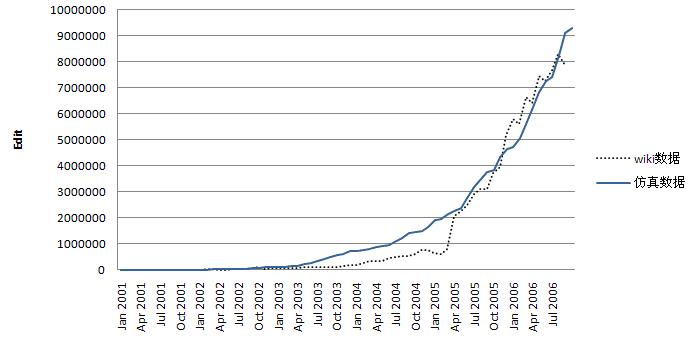
\includegraphics{07}}
  \caption{result}
\end{figure}

\section{conclusion}
\label{sec:conclusion}

 In this study, we discover that the theory of the need for
 achievement could explain the motivation factors for members in the
 virtual community of practice to participate in knowledge
 collaboration. The motivation factors include the need for
 achievement that drives individuals to achieve their goals, the need
 for affiliation that is relate to the individuals’ social
 relationship. The theory of community explains those motivation
 factors in that community members will acquire  the sense of
 belonging encouraging more communication. The simulation with system
 dynamics will help operators to fully understand the nature of
 virtual community, the need of community members, and the main
 factors affecting the success of community.

From the study, managers could learn to build the sense of identity by holding activities regularly and strengthening collective goals. First, on the individual motivation, the managers should let others know about the individual’s contribution to make the individual feel respected. Or else, managers can promote the contributors to higher level, which effectively spurs their need for achievement. The friendly atmosphere is needed to stimulate their need for affiliation, which helps members to feel themselves as part of the community. As a result, the knowledge collaboration in the virtual community of practice is promoted. On the group level, the community operators should avail the members to discuss and interact with each other on the website. The social interaction will promote the members’ sense of belonging. The operators are expected to hold regular online activities to form the common impression and group consciousness, encouraging knowledge practice by improving their sense of identity. In addition, the managers should be ready to discover the members’ dissatisfaction with the community or new needs, and improve the community service to solve the conflicts between users or from system factors. The will of users to contribute to the community could be encouraged by improving their satisfaction with the community. 
It should be noted that virtual communities are a new phenomenon with
the development of network techniques, and the related studies are at
the beginning phase with plenty of limitations. Therefore, there exist
many limitations in this study inevitably, which need to be modified
in future study. This paper aims at presenting a primary exploration
of the users’ behavior in virtual communities of practice. 

\section{Acknowledgment}
\label{sec:acknowledgment}

The work described in this paper was fully supported by the National Natural
Science Foundation of China under Grant No.70871006.

\bibliographystyle{elsarticle-num}
 \bibliography{../../bibtex/elsevier,../../bibtex/emerald,../../bibtex/chinese,../../bibtex/jstor,../../bibtex/citeseer,../../bibtex/acm,../../bibtex/wiley,../../bibtex/book,../../bibtex/thesis,../../bibtex/ebsco,../../bibtex/old,../../bibtex/ieee,../../bibtex/internet,../../bibtex/ssrn,../../bibtex/apa,../../bibtex/blackwell,../../bibtex/sage,../../bibtex/springer,../../bibtex/MESharp,../../bibtex/taylor,../../bibtex/arXiv}

\end{document}
